\setproblem{24116}

\begin{frame}[label=p2]{본선회장 (Finals)(\prob)}
\tiny

\begin{block}{문제}
JOI 국가에는 $N$개의 도시가 있으며, 각 도시는 $1$부터 $N$까지 번호가 붙어 있다. 또한 $M$개의 도로가 존재한다. 모든 도로는 서로 다른 두 도시를 연결하며, 양방향으로 통행 가능하다. JOI 국가에서는 임의의 두 도시 사이를 도로를 따라 이동하여 항상 도달할 수 있다.

JOI 국가의 모든 도로는 유료 도로이며, 각 도로마다 통행 요금이 정해져 있다. JOI 국가에서도 정보 올림피아드가 개최된다. 본선에는 각 도시의 대표 선수가 참가한다. 본선을 어떤 도시에서 개최할지 결정하고, 선수들을 해당 도시로 모으는 데 드는 비용을 계산해야 한다.

본선은 $K$개의 도시에서 개최되며, 모든 선수는 이들 중 하나의 도시로 이동해야 한다. 한 도시에 모일 수 있는 선수 수에는 제한이 없다.

선수들을 본선 개최 도시로 이동시키기 위해서는 도로를 이용한다. 통행 요금이 $c$인 도로는 한 번에 몇 명이 지나가더라도 비용은 $c$로 동일하다. 따라서 선수 이동 순서를 적절히 조정하여 여러 명이 함께 이동하도록 하면 비용을 절약할 수 있다.

본선을 개최할 도시를 적절히 선택하고, 선수들을 모을 때 드는 총 통행 요금의 합을 최소화하고자 한다.

$N$, $M$, $K$와 모든 도로의 정보가 주어졌을 때, 선수들을 본선 회장으로 모으는 데 필요한 최소 비용을 구하는 프로그램을 작성하라.
\end{block}

\begin{block}{입력}
표준 입력으로 다음과 같은 형식의 데이터가 주어진다.

첫 줄에 정수 $N$, $M$, $K$가 공백으로 구분되어 주어진다.

다음 $M$개의 줄에는 각 도로에 대한 정보가 주어진다.  
$i$번째 줄에는 정수 $A_i$, $B_i$, $C_i$가 공백으로 구분되어 주어지며, 이는 도시 $A_i$와 $B_i$를 연결하는 도로의 통행 요금이 $C_i$임을 의미한다.
\end{block}

\begin{block}{제한}
$1 \le N, M \le 100\ 000$
$1 \le K \le N$
$1 \le C_i \le 100$
\end{block}

\end{frame}

\begin{frame}{예제 입력 1}
    \begin{center}
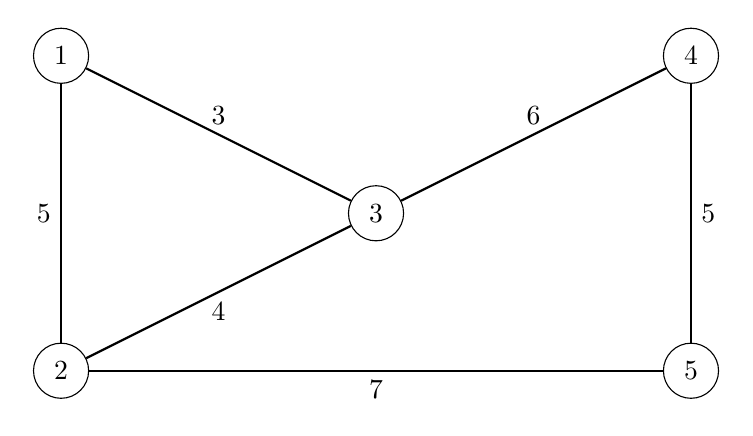
\begin{tikzpicture}[
    vertex/.style={circle, draw, minimum size=7mm},
    edge/.style={thick}
]

\node[vertex] (1) at (0,2) {1};
\node[vertex] (2) at (0,-2) {2};
\node[vertex] (3) at (4,0) {3};
\node[vertex] (4) at (8,2) {4};
\node[vertex] (5) at (8,-2) {5};

\draw[edge] (1) -- node[left] {5} (2);
\draw[edge] (1) -- node[above] {3} (3);
\draw[edge] (2) -- node[below] {4} (3);
\draw[edge] (3) -- node[above] {6} (4);
\draw[edge] (4) -- node[right] {5} (5);
\draw[edge] (2) -- node[below] {7} (5);

\end{tikzpicture}
\end{center}
\end{frame}

\begin{frame}{풀이}
\begin{itemize}
    \item $K$개의 도시 제한을 무시하고 생각하면 어떤 도시로 모이는 최소 비용은 MST의 가중치 합과 같습니다.
    \item $K$개의 도시 제한이 있으므로, MST에서 $K-1$개의 간선을 제거하여 $K$개의 연결 요소로 나누는 것이 최적입니다.
\end{itemize}
\end{frame}


\begin{frame}[fragile, allowframebreaks]{원찬혁 소스 코드}
\inputminted{java}{../src/\prob/Chanhyeok/Main.java}
\end{frame}

\begin{frame}[fragile, allowframebreaks]{손현준 소스 코드}
\inputminted{java}{../src/\prob/hyunjun/P24116.java}
\end{frame}

\begin{frame}[fragile, allowframebreaks]{김준형 소스 코드}
\inputminted{java}{../src/\prob/junhyeong/Main.java}
\end{frame}

\begin{frame}[fragile, allowframebreaks]{서민종 소스 코드}
\inputminted{java}{../src/\prob/Minjong/Main.java}
\end{frame}

\begin{frame}[fragile, allowframebreaks]{김시온 소스 코드}
\inputminted{cpp}{../src/\prob/Sion/main.cpp}
\end{frame}

\begin{frame}[fragile, allowframebreaks]{정의찬 소스 코드}
\inputminted{java}{../src/\prob/UIchan/"本選会場 (Finals)".java}
\end{frame}
